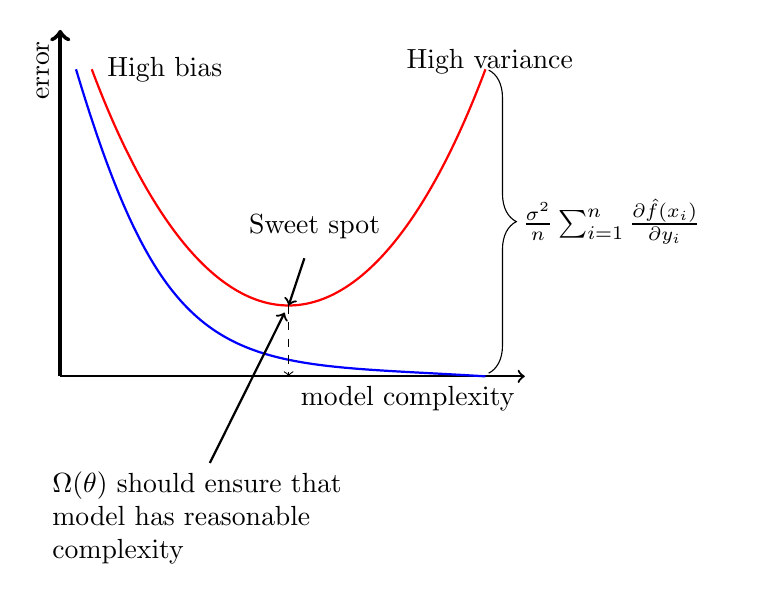
\begin{tikzpicture}
	\draw[->,thick] (4.1,-0.9)--(10,-0.9) node[below left]{model complexity};
	\draw[->,ultra thick] (4.1,-0.9)--(4.1	,3.5) node[above left,rotate=90]{error};
				
	\draw[red,thick] (4.5,3) .. controls (6,-1) and (8,-1) .. (9.5,3);
	\draw[blue,thick] (4.3,3) .. controls (5.5,-1) and (6.3,-0.7) .. (9.5,-0.9);
	\node[text width=4cm] at (6.7,3) {High bias};
	\node[text width=4cm] at (10.5,3.1) {High variance};
	\node[text width=3cm] at (8,1) {Sweet spot};
	\draw[->,thick] (7.2,0.6)--(7,0);	
	\draw[->,dashed] (7,0)--(7,-0.9);
	\draw[->,thick] (6,-2) -- (6.95,-0.09);	
	\node[text width=4cm] at (6,-2.7) {$\Omega(\theta)$ should ensure that model has reasonable complexity};
				
	%
	\draw [decorate,decoration={brace,amplitude=10pt,mirror,raise=4pt},yshift=0pt]
	(9.4,-0.86) -- (9.4,2.99) node [black,midway,xshift=1.7cm] {
		$\frac{\sigma^2}{n}\sum_{i=1}^{n}\frac{\partial\hat{f}(x_i)}{\partial y_i}$};	
\end{tikzpicture}